% STRATA: Certified Stratified Hubness for Compressed Vector Search
% VLDB/SIGIR-style systems paper -- DRAFT v0 (2026-07-24).
%
% House conventions follow paper/pca_matryoshka_pvldb.tex (acmart sigconf,
% nonacm). Figure style follows the accepted INFOCOM paper's TikZ idiom
% (boxes with rounded corners, Stealth arrows, \footnotesize, resizebox to
% column width); all figures are inline TikZ/pgfplots, no external images.
%
% SOURCES OF TRUTH (every number in this file traces to one of these):
%   docs/STRATA_RFC.md
%   docs/RESULTS_strata_phase23_gates.md
%   docs/results/strata-phase23-gates-2026-07-24/*.json
%   docs/HUBNESS_PRIMER.md
%   docs/RESULTS_multilingual_strata.md (Phase-1 run, as summarized in the RFC)
%   turboquant_pro/{strata,strata_ops,strata_remedies,duckdb_ext}.py
%   tests/{test_strata*.py,test_anatomy.py}
\documentclass[sigconf, nonacm]{acmart}
\settopmatter{printacmref=false}
\setcopyright{none}
\renewcommand\footnotetextcopyrightpermission[1]{}
\pagestyle{plain}

\usepackage{booktabs}
\usepackage{balance}
\usepackage{tikz}
\usetikzlibrary{arrows.meta,positioning,fit}
\usepackage{pgfplots}
\pgfplotsset{compat=1.17}

% Draft-level line-breaking slack: many registry/schema identifiers are
% long unbreakable \texttt tokens; give TeX room instead of overfull rules.
\setlength{\emergencystretch}{3em}

% --- DRAFT banner ---------------------------------------------------------
\newcommand{\draftbanner}{\begin{center}\fbox{\parbox{0.93\columnwidth}{\centering
\textbf{DRAFT v0 --- 2026-07-24.} Working draft; all measurements trace to
committed artifacts in
\texttt{docs/results/strata-phase23-gates-2026-07-24/}. Do not cite.}}\end{center}}

\begin{document}

\title{STRATA: Certified Stratified Hubness for Compressed Vector Search}
\subtitle{DRAFT v0 (2026-07-24) --- not for distribution}

\author{Andrew H. Bond}
\orcid{0009-0003-2599-6158}
\affiliation{%
  \institution{San Jose State University}
  \city{San Jose}\state{CA}\country{USA}}
\email{andrew.bond@sjsu.edu}

\begin{abstract}
Hubness---the emergence of nearest-neighbor ``hubs'' that appear in
hundreds of top-$k$ lists while ``anti-hubs'' appear in almost none---is a
measured property of high-dimensional retrieval, and its damage under index
compression lands precisely where aggregate recall cannot see it: on the
minority of queries whose true neighbors are anti-hubs. We present STRATA,
a system that makes hubness measurement \emph{stratified} and
\emph{certified}: the corpus is partitioned by a content-addressed area map
(\texttt{tqp-area-map/1}); every instrument reports per-area statistics
whose verdicts aggregate as \emph{min-over-strata}; thin strata
\emph{ABSTAIN} rather than pass by silence; verdict causes come from a
closed registry; and the relational surface---hub census and transit
fraction as SQL over a $k$NN edge table---\emph{refuses} to join relations
computed under different area-map digests. The components are deliberately
commodity (SQL over vectors, IVF/LOPQ-style partitioning, sixteen years of
hubness estimators); the claimed composition is the certification: columns
that know their estimator, their minimum-evidence bounds, and their
area-map identity, with refusal in the schema. We evaluate STRATA by
running its own pre-declared gates and typesetting failures like passes.
The mechanism classifier's confusion-matrix fixtures killed two simpler
designs before one survived. A four-rung measurement ladder shows CSLS
hubness correction works at the exact layer (count skew $-20\%$, Robin
Hood index $-30\%$) but is \emph{refuted} in compressed-domain scoring and
refuted \emph{identically} at reconstruction rerank---diagnosing the
bottleneck as candidate coverage, then score precision---while reranking
stored originals at depth 501 passes the $0.90$ bar in every stratum: the
codes find, the originals decide. A fragility-driven bit allocator
\emph{lowered} the measured floor (fragile-first greedy); a max-min
allocator with protected donors raised min-over-strata anti-hub recall
from $0.7251$ to $0.7697$ at an equal $3.0$ bits/row budget, and exposed
cross-area score interference as a real allocation mechanism. Finally, we
show stratified measurement is also a security instrument: per-area
centering has an adversarial dual, and a per-area mechanism shift from
density to centrality is a poisoning signature.
\end{abstract}

\keywords{vector search, hubness, quantization, certification, stratified
measurement, SQL, threat model}

\maketitle
\draftbanner

\section{Introduction}
\label{sec:intro}

A compressed vector index that reports recall@10 $= 0.98$ can be failing
one in five of its hardest queries. The mechanism is hubness: in the
dimensions embeddings actually occupy, a few corpus rows (\emph{hubs})
appear in hundreds of top-$k$ lists while a large fraction
(\emph{anti-hubs}) appear in almost none~\cite{radovanovic2010hubs}.
Queries whose true nearest neighbors are anti-hubs are the hardest
retrieval cases an index has---the signal separating the right answer from
the crowd is smallest---and quantization rounds fine distinctions away
first, so compression damage lands disproportionately on exactly those
queries while the aggregate mean stays green. \emph{Trust the tail, not
the mean} is the operating doctrine this system inherits from its parent
project's acceptance-metric work.

This paper adds a second clause: \emph{trust the tail, not the mean---in
every area}. A global anti-hub recall number has the same blindness one
level up: it can hide a collapsed stratum (a language, a tenant, a
cluster) behind healthy neighbors. Global staleness has the dual problem:
if any mutation anywhere invalidates every guarantee, guarantees become
unaffordable. STRATA (\underline{strat}ified
\underline{a}natomy) partitions measurement, remedies, operating points,
and certificates by \emph{area}, so verdicts are taken as
\textbf{min-over-strata} and mutations stale \emph{bounded regions}, not
the world.

The paper's contributions are one framework and three measured campaigns
run under it:

\begin{enumerate}
\item \textbf{The certification framework} (\S\ref{sec:framework}).
Area maps are content-addressed (\texttt{tqp-area-map/1}: canonical JSON
over the full configuration, SHA-256 digest), and an \emph{incomplete}
profile matches nothing, including itself. Per-stratum verdicts below
minimum evidence are \textbf{ABSTAIN}---reported, counted, excluded from
aggregation, and \emph{not a pass}. Verdict causes come from a closed
registry (an unregistered cause is a \texttt{KeyError} at emit time, not a
new value quietly entering an artifact). The relational surface exposes
hub census and transit fraction as SQL over a $k$NN edge table, and every
relation carries its area-map digest: helpers \emph{refuse}---not
warn---to combine relations computed under different maps.
\item \textbf{The CSLS ladder} (\S\ref{sec:csls}). Four pre-declared
gates measure where hubness correction actually works under $27.7\times$
compression. The exact layer works (count skew $-20\%$, Robin Hood index
$-30\%$). Compressed-domain application is refuted. Reconstruction rerank
is refuted with per-stratum numbers \emph{identical to four decimals}, a
coincidence that is itself the diagnosis: the bottleneck is candidate
coverage, not scoring. A depth sweep then shows coverage saturating at
$0.926$ while fidelity plateaus at $0.702$---past depth ${\sim}100$ the
ceiling is score precision---and reranking stored fp32 originals at depth
501 passes the $0.90$ bar in every stratum ($0.923$). The design
principle this ladder ends in: \emph{the codes find, the originals
decide}.
\item \textbf{Fragility allocation} (\S\ref{sec:alloc}). Spending bits on
measured fragility sounds obviously right and measurably is not:
fragile-first greedy allocation upgraded all eight of its targets and
still \emph{lowered} the min-over-strata floor by cutting unprotected
donors. A max-min allocator with protected donors raised the floor from
$0.7251$ to $0.7697$ at an equal $3.0$ bits/row budget---and revealed
\emph{cross-area score interference}: strata whose bits never changed
improved because downgraded high-headroom areas stopped stealing candidate
slots in the global top-$k$ merge.
\item \textbf{The threat model} (\S\ref{sec:threat}). Per-area centering
has an adversarial dual---a local centroid only needs to dominate a small
neighborhood, which \emph{lowers} the bar for centrality-injection
attacks~\cite{blackhole2026}---so per-area centroids are treated as
attacker-relevant encoder state that enters the identity profile.
Conversely, a per-area mechanism shift from density to centrality without
a pipeline change is a poisoning signature: the quality instrument and the
security scanner~\cite{advhubness2026} are the same tool.
\end{enumerate}

We are explicit about what is \emph{not} claimed
(\S\ref{sec:related}). SQL over vectors is
commodity~\cite{pgvector2023,raasveldt2019duckdb}; partitioned indexes
with per-cell codebooks are a decade
old~\cite{jegou2011product,kalantidis2014lopq,chen2021spann}; hubness
measurement and reduction have sixteen years of
literature~\cite{radovanovic2010hubs,schnitzer2012mutual,hara2015localized,conneau2018word}
and a standard implementation~\cite{feldbauer2020scikithubness}; and
``hubness via SQL'' is a five-line \texttt{GROUP BY} once the $k$NN graph
is an edge table. The remaining gap this paper claims is the
\emph{composition}: \textbf{certified stratified measurement with refusal
in the schema}---columns whose values know their estimator, their
$n_{\min}$, and their area-map digest, with cross-map joins refused by the
relation itself.

Every number in this paper traces to a committed JSON artifact or a CI
test fixture in the open-source repository; the evaluation protocol
(\S\ref{sec:method}) pre-declares gates and typesets failures like passes.
Three of the seven measured gates below exist \emph{because} an earlier
gate failed.

\section{Background: hubness has a mechanism}
\label{sec:background}

For a corpus $X$, query multiset $Q$, metric $d$, and depth $k$, let
$N_k(x)$ be the number of queries whose top-$k$ list contains $x$. In low
dimensions $N_k \approx k$ for everyone; in embedding dimensions the
distribution grows a long right tail whose standard scalar summary is its
skewness $S_k$~\cite{radovanovic2010hubs}. Two intuitions: distances
concentrate, so tiny systematic advantages decide top-$k$ membership; and
centrality is such an advantage---a point slightly closer to the data mean
is slightly closer to everything on average. Local density is another.

The scalar does not identify the mechanism. The parent project's anatomy
instrument (\texttt{tqp anatomy}) documents two corpora with essentially
the same skew whose hubs were completely different objects: one a smooth
tail of moderately popular points in denser regions (max $N_{10}=78$,
hubs ${\sim}8\%$ below population local scale), the other a handful of
centrality super-hubs vacuuming up lists (max $N_{10}=369$, hubs $34\%$
closer to the mean). The two mechanisms take different remedies---%
centering / localized centering~\cite{hara2015localized} for centrality,
CSLS / mutual-proximity rescaling~\cite{conneau2018word,schnitzer2012mutual}
for density---so mechanism attribution is a prescription pad, and getting
it wrong wastes the fix. Crucially, the na\"ive discriminator does not
work: $\mathrm{corr}(N_k, -d_k)$ is mechanically rank-coupled to the count
in \emph{any} corpus (it exceeds $+0.8$ on an isotropic Gaussian), which
is one of the two classifier designs our confusion matrix killed
(\S\ref{sec:confusion}).

Hubness is a property of the experiment $(X, Q, d, k)$, never of the
corpus alone: the same corpus can look mildly hubby under its own rows as
queries and extremely hubby under a real workload. Every STRATA artifact
therefore records its query battery, and corpus$\to$corpus readings are
not accepted as substitutes for workload readings.

\section{The STRATA framework}
\label{sec:framework}

\begin{figure}[t]
\centering
\resizebox{\columnwidth}{!}{%
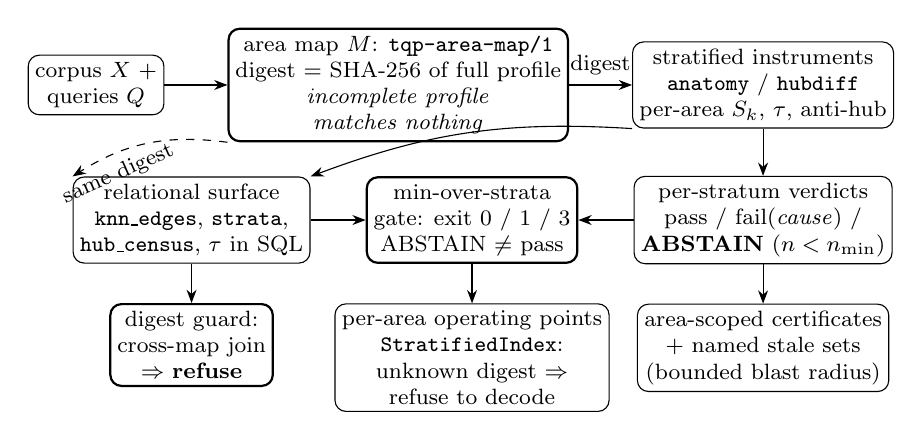
\begin{tikzpicture}[
  font=\footnotesize, node distance=4mm,
  box/.style={draw, rounded corners, align=center, minimum height=7mm,
              inner sep=2.5pt},
  hard/.style={draw, thick, rounded corners, align=center,
               minimum height=7mm, inner sep=2.5pt},
  >={Stealth[]}]
\node[box] (corpus) {corpus $X$ +\\queries $Q$};
\node[hard, right=8mm of corpus] (map)
  {area map $M$: \texttt{tqp-area-map/1}\\digest $=$ SHA-256 of full
   profile\\\emph{incomplete profile}\\\emph{matches nothing}};
\node[box, right=8mm of map] (inst)
  {stratified instruments\\\texttt{anatomy} / \texttt{hubdiff}\\per-area
   $S_k$, $\tau$, anti-hub};
\node[box, below=6mm of inst] (verdict)
  {per-stratum verdicts\\pass / fail(\emph{cause}) /\\\textbf{ABSTAIN}
   ($n<n_{\min}$)};
\node[hard, left=7mm of verdict] (min)
  {min-over-strata\\gate: exit 0 / 1 / 3\\ABSTAIN $\ne$ pass};
\node[box, left=7mm of min] (sql)
  {relational surface\\\texttt{knn\_edges}, \texttt{strata},\\
   \texttt{hub\_census}, $\tau$ in SQL};
\node[hard, below=5mm of sql] (guard)
  {digest guard:\\cross-map join\\$\Rightarrow$ \textbf{refuse}};
\node[box, below=5mm of min] (idx)
  {per-area operating points\\\texttt{StratifiedIndex}:\\
   unknown digest $\Rightarrow$\\refuse to decode};
\node[box, below=5mm of verdict] (cert)
  {area-scoped certificates\\+ named stale sets\\(bounded blast radius)};
\draw[->] (corpus) -- (map);
\draw[->] (map) -- (inst) node[midway,above]{digest};
\draw[->] (inst) -- (verdict);
\draw[->] (verdict) -- (min);
\draw[->] (inst.south west) to[bend right=12] (sql.north east);
\draw[->] (sql) -- (guard);
\draw[->] (sql) -- (min);
\draw[->] (min) -- (idx);
\draw[->] (verdict) -- (cert);
\draw[->,dashed] (map.south west) to[bend right=20]
  node[pos=0.75,below,sloped]{same digest} (sql.north west);
\end{tikzpicture}}
\caption{STRATA pipeline. A content-addressed area map stamps every
downstream artifact with its digest. Stratified instruments emit
per-stratum verdicts from a closed cause registry; thin strata ABSTAIN
(reported, counted, excluded---not a pass) and gates aggregate as
min-over-strata with exit codes $0$/$1$/$3$. The same digest guards the
relational surface (cross-map joins are refused by the relation, not
discouraged by documentation), gates per-area index decoding, and scopes
certificates to named stale sets.}
\label{fig:arch}
\end{figure}

STRATA's normative language follows RFC~2119~\cite{rfc2119}; its design
vocabulary borrows deliberately from OSPF~\cite{rfc2328} (areas, a
backbone, bounded flooding) while documenting exactly which parts of the
analogy do \emph{not} transfer (\S\ref{sec:limits}). The governing rules
are inherited from the parent project's identity discipline: uncertain
$\Rightarrow$ no verdict; an incomplete profile matches nothing, including
itself; unregistered causes raise; artifacts under different digests must
never be compared, merged, or gated together---tools refuse, not warn.
Figure~\ref{fig:arch} shows the pipeline.

\subsection{Content-addressed area maps}
\label{sec:areamap}

An \textbf{area map} $M = (A, a, a_Q, O)$ consists of area identifiers
$A=\{A_1..A_m\}$, a corpus assignment $a : X \to 2^A \setminus \emptyset$
(multi-assignment permitted), a query assignment $a_Q$ (same rule, or a
declared metadata key such as \texttt{--by language}), and a reflexive
adjacency/overlap relation $O \subseteq A \times A$ that drives staleness.

Identity is content-addressed. The profile \texttt{tqp-area-map/1} is
canonical JSON (sorted keys, tight separators, ASCII, \texttt{NaN}
forbidden) over
$\{$\texttt{profile}, \texttt{algorithm\_id}, \texttt{params},
\texttt{seed}, \texttt{corpus\_\allowbreak fingerprint},
\texttt{assignment\_\allowbreak rule},
\texttt{query\_\allowbreak assignment},
\texttt{overlap\_\allowbreak policy},
\texttt{software\_\allowbreak version}$\}$, hashed with SHA-256. Two rules give the
digest its teeth:

\begin{itemize}
\item \textbf{Incomplete matches nothing.} Any \texttt{None} field makes
the profile incomplete, and an incomplete profile is compatible with
nothing---\emph{including itself}. Unknown is contagious; there is no
``probably the same map.''
\item \textbf{Refuse, not warn.} Two artifacts computed under different
digests MUST NOT be compared, merged, or gated together. The predicate is
enforced in code (\texttt{require\_same\_map} raises the registered cause
\texttt{area\_map\_mismatch}); a serialized map whose stored digest does
not match its recomputed profile digest is refused at load as tampered.
\end{itemize}

\textbf{Boundary rule.} Nearest neighbors ignore borders. A conforming
configuration must either multi-assign boundary rows or probe
$\mathrm{home} \cup O(\mathrm{home})$ at query time; a single-area probe
under a partition (non-cover) map is a non-conforming configuration over
which certificates must not be issued. This is the part of the OSPF
analogy that fails---administrative boundaries do not exist in embedding
space---promoted from caveat to normative rule.

\subsection{Stratified instruments and area classes}
\label{sec:instruments}

For each row, the instruments split its count into intra and transit
components by whether the counting query's area matches the row's area,
yielding the \textbf{transit fraction}
$\tau(x) = N_k^{\mathrm{trans}}(x)/\max(N_k(x),1)$. Per area, the
\texttt{tqp-strata-report/1} artifact carries count skew $S_k$,
$\max N_k$, mean transit $\bar\tau$, the mechanism-attribution correlation
fields restricted to the area, and the size-stable companions (Robin Hood
index, $\mathrm{frac}(N_k > 2k)$) that survive cross-$n$ comparison. All
thresholds are \emph{fields of the report}, not constants; no number may
be claimed in prose that is not present in the artifact.

Areas are classified (reported, never hidden) into \textbf{backbone}
members (high $\tau$ and high $N_k$---transit carriers), \textbf{hub}
areas, \textbf{stub} areas (low counts in and out), and the
\textbf{not-so-hubby area} (NSHA): high intra-area skew with low
transit---local hubs, no global reach. The Phase-1 measured run on a
37-language corpus falsified both of its on-record predictions in the
informative direction: per-language $S_k$ varies far less than predicted
under BGE-M3~\cite{xiao2024bge} (the encoder homogenizes), and the trained
interlingua LaBSE~\cite{feng2022labse} does not concentrate transit on a
central core---it \emph{diffuses} it, turning 7 of 13 eligible languages
into the first measured backbone-class areas, while emergent BGE-M3 keeps
language borders (all-NSHA). The taxonomy's backbone class, speculative at
design time, exists in production encoders and is objective-dependent.

\subsection{Verdict semantics: min-over-strata and ABSTAIN}
\label{sec:verdicts}

A per-stratum verdict REQUIRES $n_i \ge n_{\min}$ corpus rows and
$|Q_i| \ge q_{\min}$ queries (defaults in every artifact below:
$n_{\min}=2000$, $q_{\min}=500$). Below either bound the verdict is
\textbf{ABSTAIN}: reported, counted under the registered cause
\texttt{stratum\_insufficient\_n}, and excluded from pass/fail
aggregation. ABSTAIN is not a pass---skewness on thin strata is noise, and
uncertain means no verdict---but it is not a silent fail either: the
report counts abstentions separately, and CI can opt in to
\texttt{--abstain-fails}. Gates aggregate as \textbf{min over eligible
(non-ABSTAIN) strata}, with exit codes $0$ (pass), $1$ (a stratum failed),
and $3$ (only-ABSTAIN).

\begin{sloppypar}
Causes and classes are a \textbf{closed registry}
(\texttt{stratum\_insufficient\_n}, \texttt{stratum\_anti\_hub\_gap},
\texttt{transit\_concentration}, \texttt{area\_map\_mismatch}; classes
\texttt{backbone}, \texttt{hub}, \texttt{NSHA}, \texttt{stub},
\texttt{plain}).
Emitting an unregistered cause raises \texttt{KeyError}. Schema fields,
cause IDs, and class names are API: additions only, with golden report
fixtures frozen in CI.
\end{sloppypar}

\subsection{The relational surface: certified hubness as SQL}
\label{sec:sql}

Once the $k$NN graph is an edge table
\texttt{knn\_edges(query\_id,} \texttt{neighbor\_id,} \texttt{rank)}, the
hub census is
in-degree---a \texttt{GROUP BY}---and the transit fraction is a join
against the \texttt{strata} relation. That much is commodity, and we say
so. The house part is that \emph{every} relation the surface registers
(\texttt{knn\_edges}, \texttt{strata}, \texttt{query\_strata},
\texttt{strata\_report}) carries an \texttt{area\_map\_digest} column, and
every helper runs a digest guard first: if the relations it is about to
join carry more than one distinct digest, it raises
\texttt{area\_map\_mismatch} and returns nothing. The replication
predicate is enforced \emph{in the schema}, not in the documentation.
The gate itself is a query: \texttt{strata\_gate} returns the failing
rows (ABSTAIN excluded, counted separately), so ``rows returned
$\Rightarrow$ exit 1'' composes with any SQL tooling the operator already
has~\cite{raasveldt2019duckdb}. The scan side streams compressed blocks
to Arrow batches, so census queries run without decompressing the corpus
into host RAM.

\subsection{Per-area operating points and bounded staleness}
\label{sec:opoints}

Per-area bits, PCA dimension, and codebooks acknowledge their LOPQ
ancestry~\cite{kalantidis2014lopq}; the new element is the allocator
input---measured per-stratum fragility (anti-hub recall), not variance
(\S\ref{sec:alloc})---and the identity gating. Record metadata gains
$\{$\texttt{area\_map\_digest}, \texttt{area\_id},
\texttt{area\_codec\_params}$\}$; a reader encountering an unknown digest
MUST refuse to decode (enumerate, don't decode). Cross-map reads are cache
misses, never best-effort; \texttt{StratifiedIndex.search} requires the
caller's digest and its refusal path is regression-tested. Areas thinner
than the requested PCA dimension clamp their per-area basis and declare it
in \texttt{area\_codec\_params}---a legitimate per-area operating point,
not a silent fallback.

Guarantees then scope naturally: the recall-contract catalog key extends
with (\texttt{area\_map\_digest}, \texttt{area\_id}), and every mutation
class has a documented worst-case stale set---a mutation in $A_i$ stales
$\mathrm{cert}(A_i)$ plus overlap neighbors; an operating-point change
stales exactly $\mathrm{cert}(A_i)$; a map recompute stales everything. A
guarantee that can go stale silently is not a guarantee; STRATA's version
has a bounded, \emph{named} blast radius, and recalibration becomes
incremental: the flapping area re-runs its measurement, the backbone does
not.

\subsection{What the OSPF analogy does not license}
\label{sec:limits}

Hierarchy, border summarization, and bounded blast radius transfer.
Administrative boundaries do not (geometry ignores them; hence the
mandatory overlap rule), and neither does link-state truth: strata are
workload-dependent ($a_Q$ matters, and corpus$\to$corpus is not a
substitute for the deployed query distribution). These limits are
normative for prose in the project's documentation, along with a banned
list (``eliminates hubness,'' ``uniform recall guaranteed'') and an
approved claim shape: \emph{``$\Delta$ measured in this artifact on this
corpus.''} This paper is written under those rules.

\section{Evaluation protocol}
\label{sec:method}

STRATA's phases each carry pre-declared gates; the evaluation below is
those gates, run and reported whether they passed or failed. Three of the
gates exist only because an earlier gate failed, and the failures carry
most of the information.

\textbf{Corpora.} (1) The \emph{Ethics 350k} sample ($n=350{,}000$,
seed~7; deployed operating point PCA-384 + 3-bit quantization,
$27.676\times$ compression, single-pass ADC search; 14 language strata of
which 7 are eligible at $n_{\min}=2000$, $q_{\min}=500$). (2) The public
paired \emph{Gutenberg} rung, BGE-M3 arm ($n=150{,}067$ rows, 20 language
strata, 14 eligible). Ground truth throughout is exact $k$NN on the given
vectors at $k=10$; the fidelity instrument is the stratified differential
oracle (\texttt{hubdiff}) with anti-hub recall gated at $0.90$ over
bottom-decile rows of the \emph{global} count distribution (a stratum
cannot vote itself out of having anti-hubs). Every report artifact carries
its area-map digest, estimator, thresholds, and software version; the
artifacts are committed in the repository at
\texttt{docs/results/strata-}\allowbreak\texttt{phase23-gates-2026-07-24/}.

\section{The mechanism classifier and the confusion matrix that killed two designs}
\label{sec:confusion}

Mechanism attribution (centrality vs.\ density) selects the remedy, so a
misclassification wastes the fix. The classifier is validated by a
confusion matrix of four constructed fixture families, one per cell of the
prescription pad, each run at three seeds (Table~\ref{tab:confusion}).
Two earlier designs died against these fixtures before the current one
survived:

\begin{enumerate}
\item \textbf{Corpus-wide correlation thresholds.} Classifying on the
correlation $\mathrm{corr}(N_k, -d_k)$ fails because it is coupled
mechanically to the count in any corpus---it exceeds $+0.8$ even on an
isotropic Gaussian---so it cannot discriminate mechanisms at all.
\item \textbf{Symmetric percentile thresholds.} Typing each hub by
independent percentile cuts on centrality and density fails on the
dominance structure: a hub in the deep centrality tail has a small $d_k$
\emph{because} it is central (apparent density is implied by centrality),
so density-typing must be conditioned on \emph{not} being central.
\end{enumerate}

The surviving design types each hub hierarchically by its population
percentiles---deep-centrality-tail hubs are central regardless of their
density; dense-but-not-central is the healthy real-corpus pattern---and
abstains entirely when there is no material hub tail
($\max N_k < 2.5k$): noise hubs get no prescription. One scope limit is
declared rather than patched: at global scope, \emph{locally} central hubs
read as dense (a point too close to everything in its own region has a
small $d_k$ globally), and CSLS is the correct global remedy for both.
Splitting them apart is precisely per-area work---the fixture that
motivates STRATA.

\begin{table}[t]
\caption{The classifier's confusion matrix: four fixture families
$\times$ three seeds, all cells required to hold in CI
(\texttt{tests/test\_anatomy.py}). These fixtures killed the two designs
described in \S\ref{sec:confusion}.}
\label{tab:confusion}
\small
\begin{tabular}{@{}p{2.35cm}p{2.9cm}p{2.5cm}@{}}
\toprule
fixture construction & required attribution & required evidence \\
\midrule
unit shell + points planted at the center &
\texttt{centrality}; prescription: centering &
$\mathrm{hub\_frac\_central}$ $= 1.0$ \\[2pt]
off-center shells, each with planted \emph{local} centers &
\texttt{density}; prescription: CSLS &
dense-noncentral frac $\ge 0.75$; central frac $= 0$ \\[2pt]
density corpus with origin shell also center-planted &
\texttt{mixed} &
both fractions $\ge 0.25$ \\[2pt]
constant-density ring (negligible hubness) &
\texttt{unclear}: attribution \emph{abstains} &
$\max N_k < 2.5k$; ``no material hub tail'' \\
\bottomrule
\end{tabular}
\end{table}

The differential oracle is validated the same way: a fixture corrupts only
queries whose true nearest neighbor is an anti-hub and CI requires
aggregate recall to stay above $0.75$ while anti-hub recall collapses
below $0.30$---the exact failure shape aggregate metrics cannot see, held
as a permanent regression test.

\section{The CSLS ladder: where correction actually works}
\label{sec:csls}

CSLS~\cite{conneau2018word} (and mutual
proximity~\cite{schnitzer2012mutual}) corrects density-mechanism hubness
with one precomputed scalar per record: $r_k(x)$, the mean similarity of
$x$ to its $k$ nearest neighbors, subtracted from the raw score at ranking
time. One float32 per record makes it a natural optional trailer in the
storage format (registered ID \texttt{0x10},
\texttt{hubness-scalar/1}, carrying its own hash; unknown-optional
$\Rightarrow$ skip, so old readers remain conformant). The question the
ladder answers: \emph{at which layer of a compressed search stack does the
correction survive?} All rungs run on Ethics 350k at the deployed
$27.676\times$ operating point, gated at min-over-strata anti-hub recall
$\ge 0.90$.

\subsection{Gate A: failed by design error}

The first gate scored CSLS-rescored ADC rankings against
\emph{uncorrected} exact-cosine ground truth. Anti-hub recall ``dropped''
by roughly $0.32$ in every stratum (min-over-strata $0.437$ at $w=1.0$,
$0.571$ at $w=0.5$). The diagnosis: the gate conflated two questions.
CSLS is a \emph{different ranking objective}; scoring it against cosine
truth measures disagreement, not damage. The gate design, not the remedy,
failed first---kept on the scoreboard as the reason Gate A$'$ exists.

\subsection{Gate A$'$: the two questions separated}

\textbf{A$'$1 --- does CSLS reduce hubness on the exact graph? Yes.}
Table~\ref{tab:a1} shows the exact-layer effect at $w=1.0$: every
hub-tail statistic improves. The $r_k$ scalar earns its trailer---measured
hub-tail reduction on this corpus at every statistic.

\begin{table}[t]
\caption{Gate A$'$1: exact-layer CSLS vs.\ cosine, Ethics 350k, $k=10$,
$w=1.0$ (artifact \texttt{phase2\_efficacy\_v2.json}).}
\label{tab:a1}
\small
\begin{tabular}{@{}lccc@{}}
\toprule
statistic & cosine graph & CSLS graph & $\Delta$ \\
\midrule
count skew & 3.970 & 3.177 & $-20\%$ \\
count max & 287 & 213 & $-26\%$ \\
Robin Hood index & 0.372 & 0.261 & $-30\%$ \\
$\mathrm{frac}(N_k > 2k)$ & 0.117 & 0.079 & $-33\%$ \\
\bottomrule
\end{tabular}
\end{table}

\textbf{A$'$2 --- does compressed CSLS reproduce exact CSLS? No.}
Rescoring ADC scores with $r_k$ and judging against exact-CSLS truth:
min-over-strata anti-hub recall $0.663$ against the $0.90$ bar; all 7
eligible strata fail; per-stratum recalls $0.62$--$0.69$---substantially
\emph{worse} fidelity than the uncorrected path ($0.76$--$0.84$). The
reading: CSLS promotes exactly the isolated, fine-distinction rows that
$27.7\times$ quantization damages first, so the corrected ranking is
\emph{harder} to reproduce from compressed codes than the uncorrected one.
Consequence (normative): the \texttt{hubness-scalar/1} trailer semantics
stay provisional, and no unconditional improvement claim is made.

\subsection{Gate A$''$: rerank refuted---identically}

The natural rescue is two-stage: fetch ADC candidates (depth 51, the
deployed single pass), rerank by cosine on \emph{reconstructed} candidates
minus $r_k$, judge against exact-CSLS truth. Measured: min-over-strata
anti-hub recall $\mathbf{0.6627}$---\emph{identical to A$'$2 to four
decimals}, with per-stratum values matching within $\pm 0.0001$.

The identity is the finding. Moving CSLS from compressed-domain scoring to
reconstruction rerank changed \emph{nothing}, so the bottleneck is not the
scoring layer---it is \textbf{candidate coverage}. Exact-CSLS's true
neighbors (isolated, low-$r_k$ rows) frequently do not appear in the plain
ADC top-51 at all, and no rerank scheme can recover a candidate that was
never fetched. (Reconstruction carries the same information as the codes,
so this rung also pre-answers ``rerank harder'': there is nothing more in
the codes to extract.)

\subsection{Gate A$'''$: coverage saturates, fidelity does not follow}

One ADC sweep at depth 501, every smaller depth a prefix, CSLS rescore at
each depth (Figure~\ref{fig:ladder}, artifact
\texttt{phase2\_depth\_curve.json}): coverage of the CSLS truth climbs
$0.696 \to 0.788 \to 0.861 \to 0.926$ (23 points), while fidelity gains
$+0.033$, then $+0.004$, then $+0.002$---a plateau at $0.702$ against
coverage $0.926$. The diagnosis is therefore \emph{layered}: at depth 51
the ceiling is coverage (A$''$'s finding); past depth ${\sim}100$ the
ceiling becomes \textbf{score precision}---the true neighbor is \emph{in}
the candidate list and the $27.7\times$ scores are too coarse to place it.
Deeper candidates alone are not a remedy: $10\times$ the scan depth buys
$+0.039$ fidelity.

\subsection{Gate A$''''$: the originals-rerank storage trade passes}

The one remaining lever is reranking against stored fp32 originals
(4096~B/row on top of the 148~B/row compressed record)---the true CSLS
objective evaluated on the candidate list. The pre-declared prediction
confirmed exactly: fidelity equals coverage at every depth
($0.702/0.792/0.861/\mathbf{0.923}$ at depths $51/101/201/501$ vs.\
coverage $0.696/0.788/0.861/0.926$; artifact
\texttt{phase2\_originals\_trade.json}), and at depth 501 zero strata
fail the $0.90$ bar.

\begin{figure}[t]
\centering
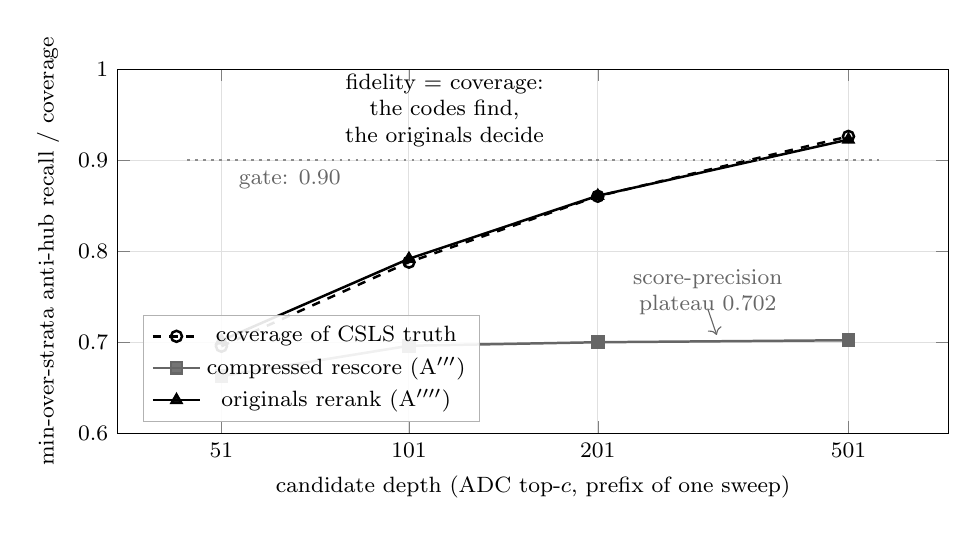
\begin{tikzpicture}
\begin{axis}[
  width=\columnwidth, height=6.2cm,
  xmode=log, log ticks with fixed point,
  xtick={51,101,201,501}, xticklabels={51,101,201,501},
  xlabel={candidate depth (ADC top-$c$, prefix of one sweep)},
  ylabel={min-over-strata anti-hub recall / coverage},
  ymin=0.60, ymax=1.0,
  grid=major, grid style={black!12},
  legend style={at={(0.03,0.03)}, anchor=south west, font=\footnotesize,
                draw=black!30, fill=white, fill opacity=0.9,
                text opacity=1},
  every axis plot/.append style={line width=0.9pt},
  tick label style={font=\footnotesize},
  label style={font=\footnotesize}]
\addplot[black, dashed, mark=o, mark options={solid}]
  coordinates {(51,0.6956) (101,0.7881) (201,0.8606) (501,0.9264)};
\addlegendentry{coverage of CSLS truth}
\addplot[black!60, mark=square*]
  coordinates {(51,0.6627) (101,0.6961) (201,0.7000) (501,0.7022)};
\addlegendentry{compressed rescore (A$'''$)}
\addplot[black, mark=triangle*]
  coordinates {(51,0.7019) (101,0.7918) (201,0.8611) (501,0.9229)};
\addlegendentry{originals rerank (A$''''$)}
\addplot[black!45, dotted, line width=0.7pt, domain=45:560] {0.90}
  node[pos=0.06, below right, font=\footnotesize, black!60] {gate: $0.90$};
\node[font=\footnotesize, align=center, black!60]
  at (axis cs:300,0.755) {score-precision\\plateau $0.702$};
\draw[->, black!60] (axis cs:300,0.737) -- (axis cs:310,0.708);
\node[font=\footnotesize, align=center]
  at (axis cs:115,0.955) {fidelity $=$ coverage:\\the codes find,\\the
  originals decide};
\end{axis}
\end{tikzpicture}
\caption{The CSLS ladder's depth sweep (Ethics 350k, $27.676\times$,
$w=1.0$; artifacts \texttt{phase2\_depth\_curve.json},
\texttt{phase2\_originals\_trade.json}). Candidate coverage of the
exact-CSLS truth saturates ($0.926$ at depth 501) while compressed-domain
rescoring plateaus at $0.702$---past depth ${\sim}100$ the binding
constraint is score precision, not coverage. Reranking stored fp32
originals tracks coverage at every depth and passes the $0.90$
min-over-strata gate at depth 501 ($0.923$, zero failing strata).}
\label{fig:ladder}
\end{figure}

\subsection{The complete menu, and the principle}

All three deployment options are now measured, none extrapolated:
(1)~\textbf{exact-layer CSLS}---free, works (A$'$1);
(2)~\textbf{compressed-path CSLS}---refuted three ways (A$'$2, A$''$,
A$'''$: first coverage-limited, then score-precision-limited);
(3)~\textbf{paid CSLS}---deployed codes + stored originals + depth-501
rerank clears the bar in every stratum. This is the project's tiered
rerank architecture doing for the \emph{corrected} ranking what it
previously did for the plain one at the billion-row fleet run:
\textbf{the codes find, the originals decide}. Compressed codes are a
candidate generator; verdicts belong to a representation that still
contains the fine distinctions the verdict is about.

\section{Fragility allocation: raising the floor without digging under it}
\label{sec:alloc}

Per-area operating points make capacity a policy variable: which strata
get 4 bits and which get 2, at a fixed corpus-wide budget? STRATA's
allocator input is measured fragility---per-stratum anti-hub recall from
the differential oracle---rather than variance. Both gates run on the
public Gutenberg rung (BGE-M3 arm, $150{,}067$ rows, 20 language strata,
14 eligible) at an equal budget of $3.0$ bits/row against the uniform
3-bit baseline, whose min-over-strata anti-hub recall is $0.7251$
(spanish).

\subsection{Gate B: fragile-first greedy fails, instructively}

The obvious allocator upgrades the most fragile strata first while the
row-weighted mean stays within budget. It did exactly what it was told:
all eight of its 4-bit targets improved ($+0.004$ to $+0.034$). It also
cut its unprotected donors below the old floor---english
$0.7546 \to 0.6856$, greek $-0.062$, latin $-0.053$---dragging
min-over-strata down to $0.6856$, \emph{below} the uniform baseline it was
meant to improve. It flattened the distribution and lowered the minimum.
The lesson, stated as the gate's epitaph: \emph{min-over-strata is not
improved by spending on the weak; it is improved by not digging under the
floor.}

\subsection{Gate B2: max-min with protected donors passes}

The redesigned allocator optimizes the floor directly, under declared
rules: recipients are the fragile half (below the median baseline recall),
upgraded most-fragile-first; donors need headroom $\ge 0.06$ over the
baseline \emph{minimum} (the one-bit penalty Gate B measured) and give at
most one step; unfundable upgrades revert their donations; ABSTAIN strata
hold the uniform width. At the same budget (achieved $2.995$ bits/row):

\begin{itemize}
\item \textbf{min-over-strata anti-hub recall: $0.7251 \to 0.7697$}
($+0.045$), no stratum below the old minimum---the pre-declared PASS
condition (artifact \texttt{phase3\_trade\_v2.json}).
\item Every recipient-half stratum improved (spanish $+0.047$, swedish
$+0.054$, italian---the one funded 4-bit upgrade---$+0.050$); protected
latin \emph{improved} ($+0.035$) instead of being cut; donors paid at most
$-0.014$ (greek); two donors (chinese, esperanto) improved despite their
downgrades.
\end{itemize}

\begin{figure*}[t]
\centering
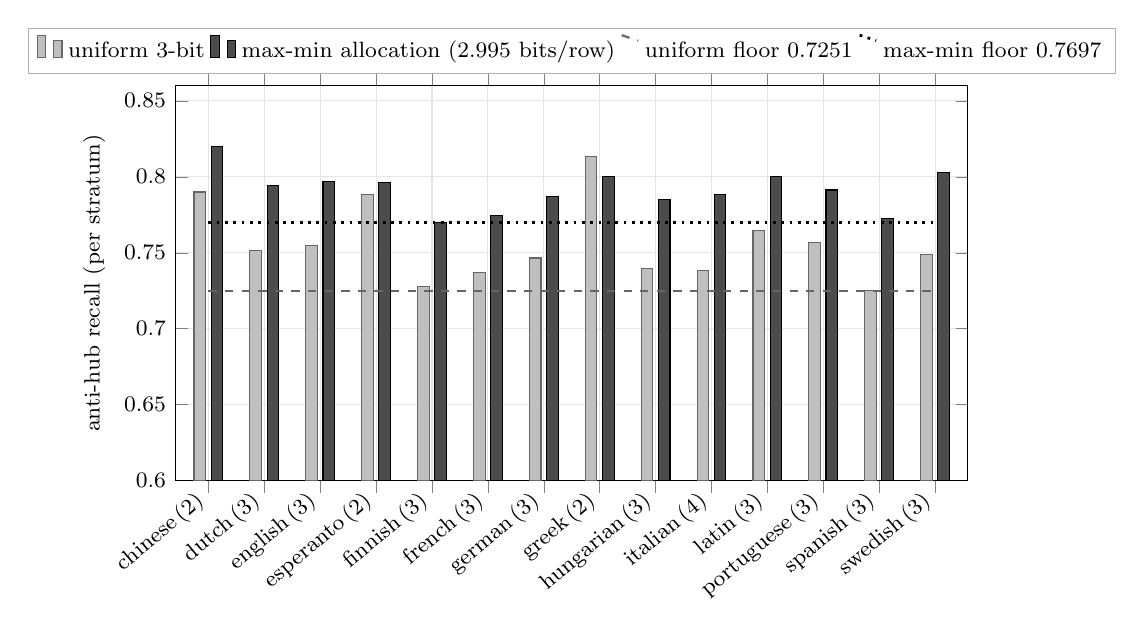
\begin{tikzpicture}
\begin{axis}[
  width=0.96\textwidth, height=6.6cm,
  ybar, bar width=4.2pt,
  ymin=0.60, ymax=0.86,
  ylabel={anti-hub recall (per stratum)},
  symbolic x coords={chinese,dutch,english,esperanto,finnish,french,german,
    greek,hungarian,italian,latin,portuguese,spanish,swedish},
  xtick=data,
  xticklabels={chinese\,(2),dutch\,(3),english\,(3),esperanto\,(2),
    finnish\,(3),french\,(3),german\,(3),greek\,(2),hungarian\,(3),
    italian\,(4),latin\,(3),portuguese\,(3),spanish\,(3),swedish\,(3)},
  x tick label style={rotate=40, anchor=east, font=\footnotesize},
  tick label style={font=\footnotesize},
  label style={font=\footnotesize},
  legend style={at={(0.5,1.03)}, anchor=south, legend columns=4,
                font=\footnotesize, draw=black!30},
  grid=major, grid style={black!10},
  enlarge x limits=0.045]
\addplot[fill=black!25, draw=black!60]
  coordinates {(chinese,0.7900) (dutch,0.7514) (english,0.7546)
    (esperanto,0.7885) (finnish,0.7280) (french,0.7368) (german,0.7466)
    (greek,0.8135) (hungarian,0.7396) (italian,0.7385) (latin,0.7647)
    (portuguese,0.7565) (spanish,0.7251) (swedish,0.7486)};
\addlegendentry{uniform 3-bit}
\addplot[fill=black!70, draw=black]
  coordinates {(chinese,0.8200) (dutch,0.7944) (english,0.7968)
    (esperanto,0.7962) (finnish,0.7697) (french,0.7745) (german,0.7868)
    (greek,0.8000) (hungarian,0.7849) (italian,0.7885) (latin,0.8000)
    (portuguese,0.7913) (spanish,0.7725) (swedish,0.8029)};
\addlegendentry{max-min allocation (2.995 bits/row)}
\addplot[black!60, dashed, sharp plot, line width=0.8pt]
  coordinates {(chinese,0.7251) (swedish,0.7251)};
\addlegendentry{uniform floor 0.7251}
\addplot[black, dotted, sharp plot, line width=1.0pt]
  coordinates {(chinese,0.7697) (swedish,0.7697)};
\addlegendentry{max-min floor 0.7697}
\end{axis}
\end{tikzpicture}
\caption{Gate B2: per-stratum anti-hub recall under the uniform 3-bit
baseline vs.\ the max-min allocation with protected donors, Gutenberg rung
(BGE-M3 arm, $150{,}067$ rows; 14 eligible strata of 20; artifact
\texttt{phase3\_trade\_v2.json}). Parenthesized tick labels give the
allocated bits per stratum (italian is the one funded 4-bit upgrade;
chinese, esperanto, and greek are 2-bit donors). The floor rises
$0.7251 \to 0.7697$ at an equal $3.0$ bits/row budget with no stratum
below the old minimum; donors pay at most $-0.014$ (greek), and unchanged
3-bit strata improve $+0.03$--$0.05$---the cross-area score interference
of \S\ref{sec:interference}.}
\label{fig:alloc}
\end{figure*}

\subsection{Cross-area score interference}
\label{sec:interference}

The unplanned finding is visible in Figure~\ref{fig:alloc}: strata whose
bit width \emph{never changed} improved by $+0.03$--$0.05$. The mechanism
is real and the uniform baseline could not have shown it: the global
top-$k$ merges ADC scores \emph{across} areas, so a high-headroom area's
coarsely-quantized rows compete for candidate slots against every other
area's true neighbors. Downgrading the high-headroom donors reduced their
rows' ability to steal those slots. \textbf{Allocation is not
per-area-local}: a bit spent (or saved) in one stratum moves retrieval
quality in strata it never touched.

\subsection{Limits and allocator defects, on the record}

A structural limitation, stated plainly: with this corpus's donor capacity
(${\sim}8$k eligible donor rows), the largest fragile strata (spanish 10k;
finnish, french, german 15k each) were individually unfundable; the
allocator funded what it could and the floor still rose. On donor-scarce
corpora the safe answer converges toward uniform---that convergence is a
feature, not a failure mode.

The gates also found (and CI now pins) three allocator defects:
fragile-first greedy lowers the floor (Gate B, replaced by max-min); the
first max-min implementation leaked donations when a recipient was
unfundable---donors cut, nobody upgraded, strictly worse than uniform---and
gave up rather than trying cheaper recipients (donations now revert and
iteration continues); and the stratified index crashed on areas thinner
than the PCA dimension (per-area dimension now clamps and declares itself
in \texttt{area\_codec\_params}).

\section{Threat model: measurement as intrusion detection}
\label{sec:threat}

Two 2026 results moved hubness from a retrieval-quality concern to a
security surface, and both validate the mechanism taxonomy of
\S\ref{sec:background}. The Black-Hole Attack~\cite{blackhole2026}
injects a handful of vectors near the embedding-space centroid---%
exploiting centrality-mechanism hubness on real BGE embeddings---and
hijacks the vast majority of top-10 results; cluster-wise centroids
\emph{amplify} the attack, because a local centroid only needs to dominate
a small neighborhood. The Adversarial Hubness
Detector~\cite{advhubness2026} ships an open-source hubness-poisoning
scanner across FAISS/Pinecone/Qdrant/Weaviate using MAD-based count
z-scores and cross-cluster retrieval-spread analysis---the latter a
convergent cousin of STRATA's transit fraction $\tau$.

STRATA draws two normative consequences.

\textbf{Per-area centering has an adversarial dual.} Localized
centering~\cite{hara2015localized} at region scale is the natural remedy
for centrality-mechanism areas---and it \emph{lowers the bar} for
centrality-injection attacks, for exactly the reason it works. The
framework therefore treats stored per-area centroids as attacker-relevant
encoder state: they enter the identity profile (changing them is an epoch
event that moves the digest, never a silent tweak), and Phase-2 remedies
are never deployed as write-path trust.

\textbf{Mechanism shift is a poisoning signature.} A planted super-hub
\emph{is} a centrality hub, so the anatomy report doubles as a monitoring
instrument: a sudden per-area mechanism shift from density to centrality,
or a jump in $\mathrm{hub\_frac\_central}$, without a pipeline change is
an investigation, not a re-quantization. The monitoring hook is a diff of
the \texttt{mechanism} and $\mathrm{hub\_frac\_central}$ fields per area
across index mutations---which the digest discipline makes meaningful,
since both sides of the diff are guaranteed to be measurements of the same
experiment. The quality instrument and the security scanner are the same
tool; the exact-layer $r_k$ scalar's measured value today
(\S\ref{sec:csls}) is A$'$1's hub-tail reduction \emph{plus} this
monitoring signal, not compressed-path retrieval correction.

\section{Related work and honest positioning}
\label{sec:related}

\textbf{Every component is commodity, and the decomposition is stated
before a reviewer states it for us.} SQL over vector search is shipped by
pgvector~\cite{pgvector2023}, DuckDB-based
stacks~\cite{raasveldt2019duckdb}, and Vector-SQL
systems~\cite{TODO-myscale-vectorsql}. Partitioned indexes are
IVF~\cite{jegou2011product,johnson2019faiss}; per-cell codebooks are
LOPQ~\cite{kalantidis2014lopq}; boundary duplication is
SPANN~\cite{chen2021spann}; emergent hub backbones are HNSW's upper
layers~\cite{malkov2020hnsw}. Hubness emergence is Radovanovi\'c et
al.~\cite{radovanovic2010hubs}; the reduction canon is mutual
proximity~\cite{schnitzer2012mutual}, localized
centering~\cite{hara2015localized}, and CSLS~\cite{conneau2018word}, with
\texttt{scikit-hubness}~\cite{feldbauer2020scikithubness} as the standard
implementation of measurement and reduction. ``Hubness via SQL'' is a
five-line \texttt{GROUP BY} once the $k$NN graph is an edge table. The
security community is converging from the adversarial
side~\cite{blackhole2026,advhubness2026}, shipping scanners.

What none of these ship, and what this paper claims, is the
\emph{composition}: \textbf{a relational surface over certified stratified
hubness}---areas that are hubness-diagnosed, fragility-allocated,
identity-versioned, and carry per-region guarantees with bounded, named
staleness; columns whose values know their estimator, their
minimum-evidence bounds, and their area-map digest; and cross-map joins
refused by the relation itself rather than discouraged by documentation.
The detectors ship scanners; the databases ship \texttt{DISTANCE()}; the
composition is the claim. No ``first'' claim is made beyond it, per the
project's positioning rules; a completed literature-check notebook is a
precondition for any stronger wording.

\section{Limitations}
\label{sec:limitations}

The measured campaigns cover two corpora (350k and 150k rows) and one
compressed operating-point family; the approved claim shape---``$\Delta$
measured in this artifact on this corpus''---is the only claim shape used,
and no cross-corpus generalization is asserted. The originals-rerank pass
is a storage trade (4096~B/row of fp32 originals against 148~B/row codes)
whose latency cost at deployment scale is characterized in the companion
systems work, not here. The Gate-B2 allocator's response model is one
measured bit-step; two-step penalties are unmeasured, and the allocator
refuses to extrapolate them by construction. Overlap policy
(multi-assignment vs.\ adjacent-probe) is a recorded open decision:
Phase-1/2/3 artifacts here use single-assignment maps, which is a
non-conforming configuration for Phase-4 certificates and is labeled as
such in every artifact. Certificate catalog wiring beyond the normative
core (contract keys, stale sets---implemented and tested) remains future
work.

\section{Conclusion}
\label{sec:conclusion}

STRATA turns hubness measurement from a scalar into a certified, spatial
instrument: content-addressed area maps whose incomplete profiles match
nothing, min-over-strata verdicts whose thin strata ABSTAIN rather than
pass, closed cause registries, and a relational surface that refuses
cross-map joins in the schema. Run against its own pre-declared gates, the
framework produced findings its unstratified predecessors could not have
seen: a confusion matrix that killed two classifier designs; a
four-decimal coincidence that located a bottleneck (coverage, then score
precision) and ended in a deployable principle---the codes find, the
originals decide; an ``obviously correct'' allocator measurably digging
under the floor it was meant to raise, and its max-min replacement raising
that floor $0.7251 \to 0.7697$ at equal budget while exposing cross-area
score interference; and a threat model in which the measurement instrument
doubles as the intrusion detector. Trust the tail, not the mean---in every
area.

\begin{acks}
DRAFT v0. Artifacts, code, and test fixtures:
\url{github.com/ahb-sjsu/turboquant-pro} (MIT). All measurements in
this paper are committed under
\texttt{docs/results/strata-}\allowbreak\texttt{phase23-gates-2026-07-24/}
with their area-map digests; the framework and gate definitions are
\texttt{docs/STRATA\_RFC.md} and
\texttt{docs/RESULTS\_}\allowbreak\texttt{strata\_phase23\_gates.md}.
\end{acks}

\balance
\bibliographystyle{ACM-Reference-Format}
\bibliography{strata_systems}

\end{document}
